\begin{frame}{Agents}
    \centering
    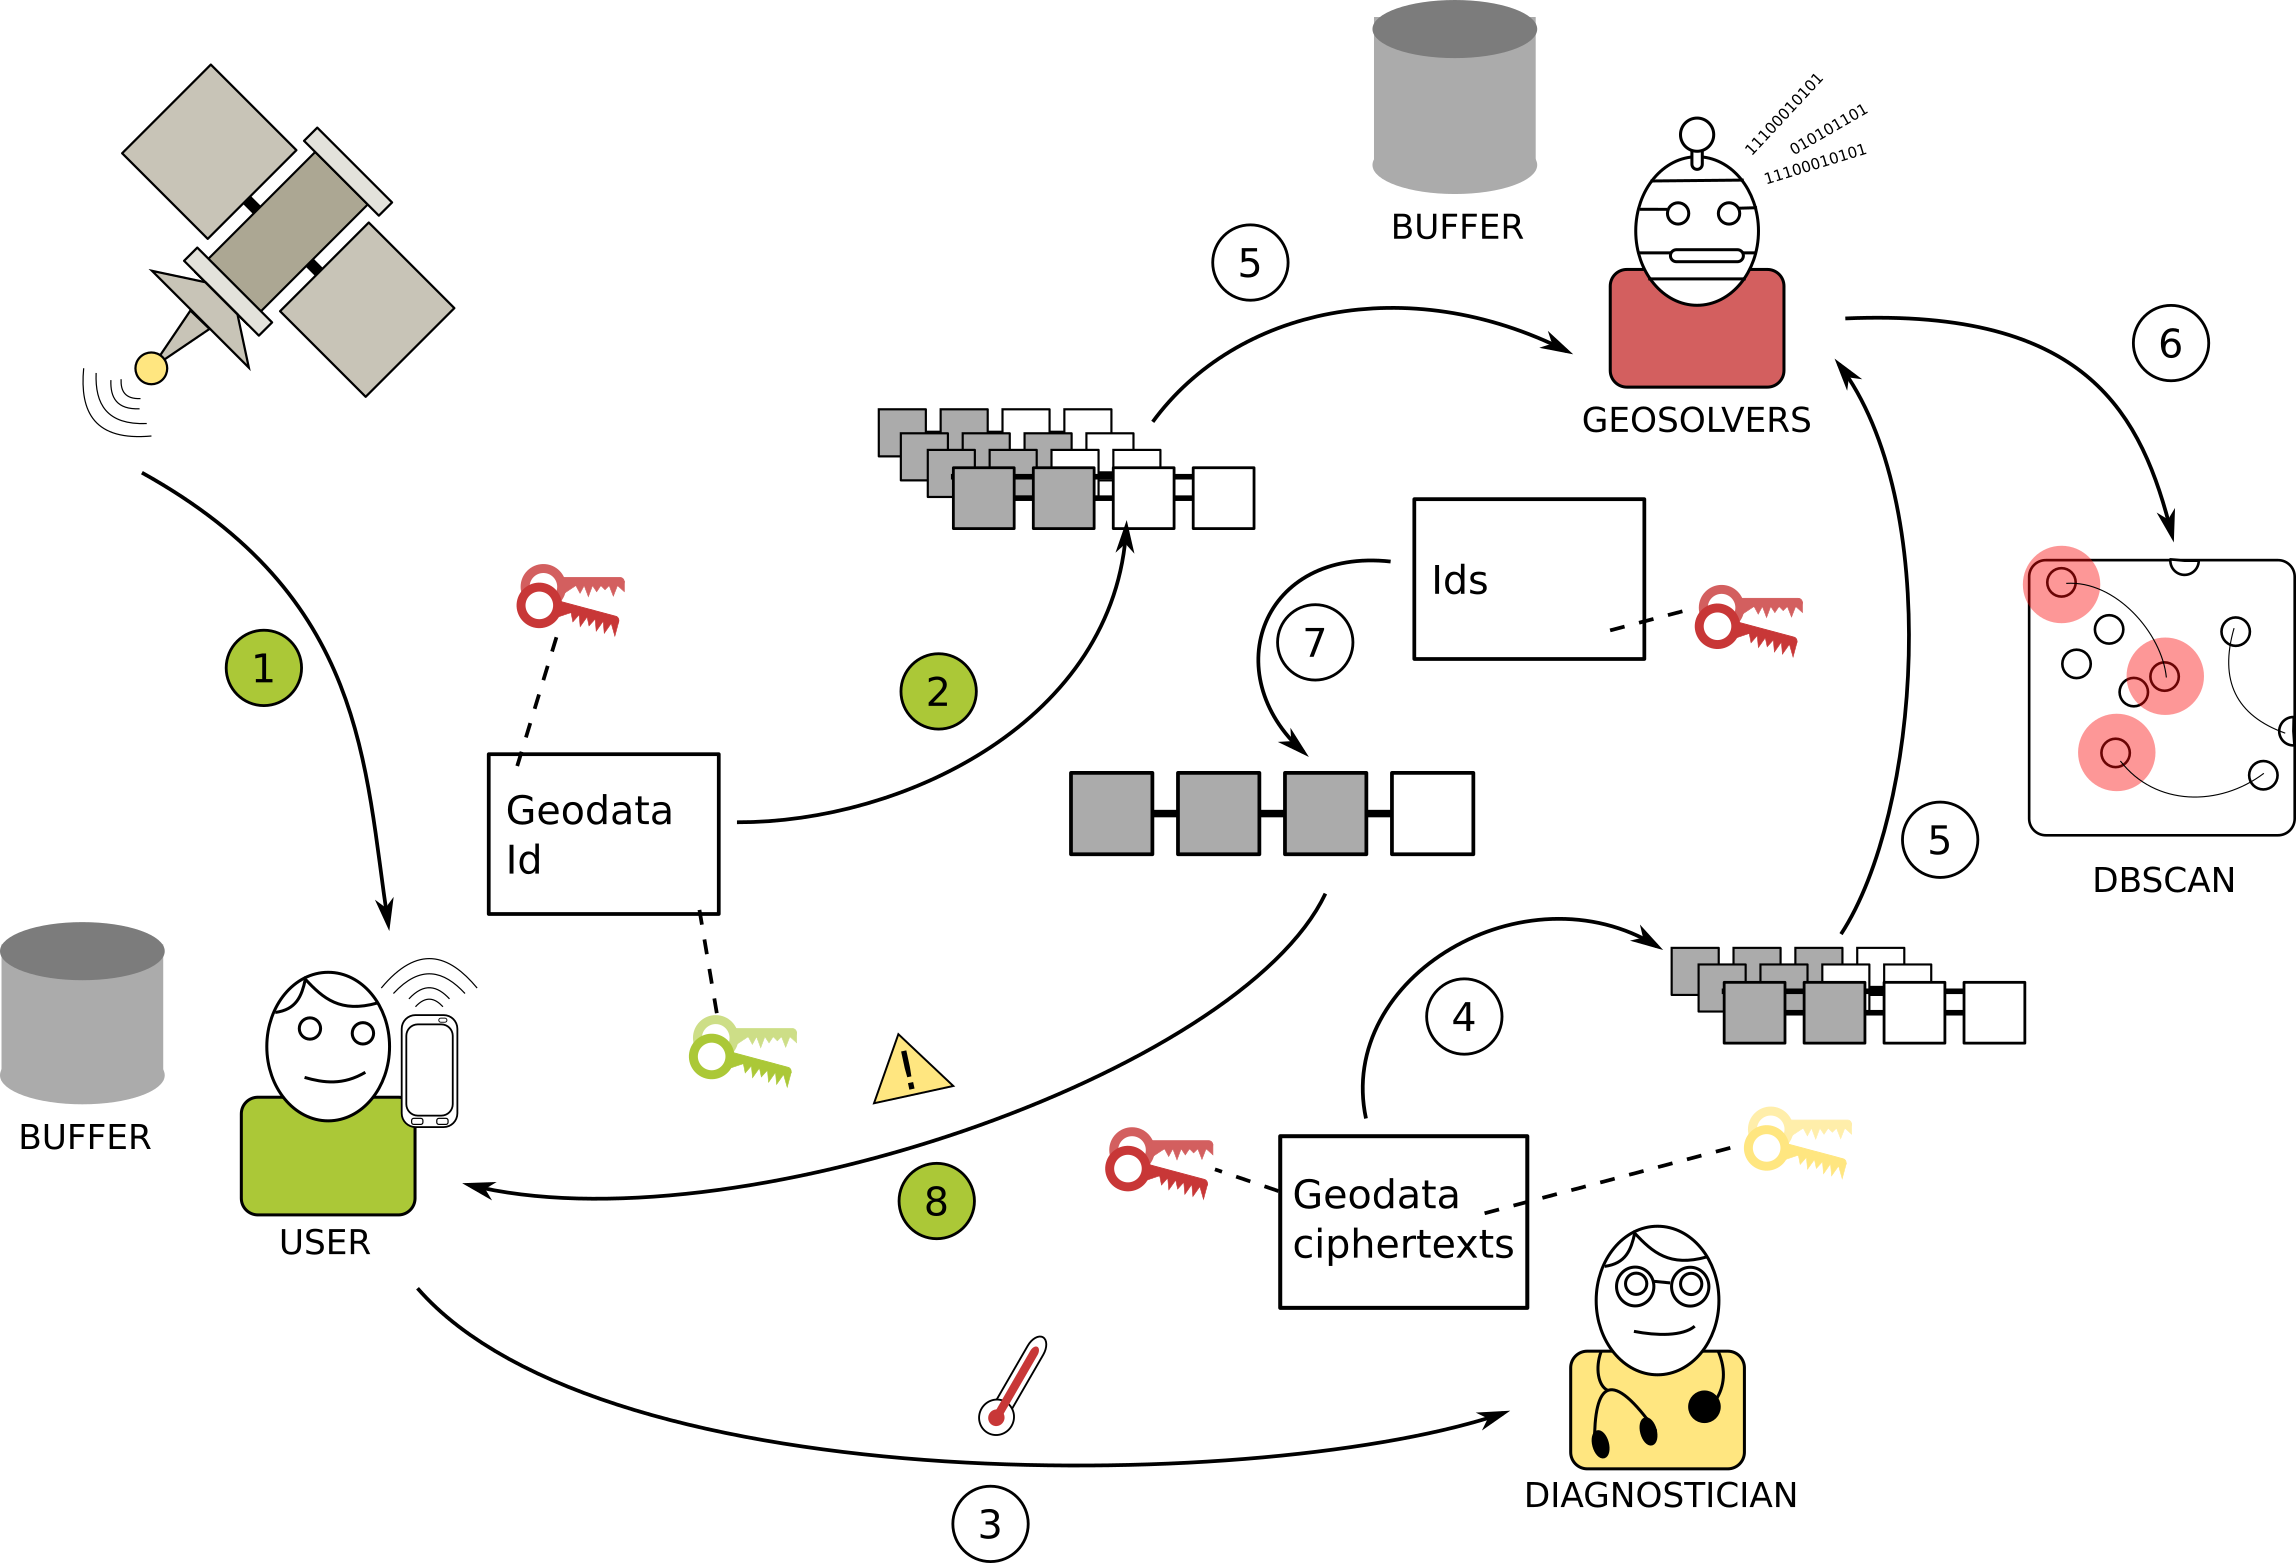
\includegraphics[width=0.95\linewidth]{images/design_agents.png}
\end{frame}

\begin{frame}{Agents}
    \begin{block}{Characteristics}
        \begin{itemize}
            \item \textbf{Generic individuals} moving in the space
            \item Have a \textbf{unique ID}, which is randomly generated
            \item Own their personal \textbf{MAM channel}
            \item Own a pair of \textbf{keys} to encrypt data for the geosolver
            \item Own a \textbf{shared key} to read data from the geosolver
        \end{itemize}
    \end{block}
    
    \vspace{-10pt}
    
    \begin{columns}[T]
    \column{0.60\linewidth}
        \begin{block}{Tracking Procedure}
            Agents keep their geospatial data in a cache, which is updated every slot of time, then, whenever it is full:
            \begin{itemize} 
                \item [1.] Its content is encrypted using the agents' private key and the geosolver's public key
                \item [2.] The obtained ciphertext is signed using the agents' private key
                \item [3.] Then, agents append this ciphertext to the MAM channel along with the respective signature and both their public key and their ID
            \end{itemize}
        \end{block}
        
        \column{0.36\linewidth}
        \begin{block}{Notification Procedure}
            When new data is posted on the geosolver's MAM channel, the agents fetch them, then:
            \begin{itemize}
                \item [1.] Verify the correctness of the signature
                \item [2.] Decrypt the data using the shared private key
                \item [3.] Check if their ID is in the list of possible infected
            \end{itemize}
        \end{block}
    \end{columns}
\end{frame}